\section{\uppercase{Design and Architecture}}
\label{sec:architecture}

% principles
\noindent Workflow and requirements described in the previous section have been received in \emph{Metior}, a prototypal application serving as proof of concept. 
It is strongly web based
it runs in a modern web browser, thus maximizing accessibility, 
it is built using React by Facebook and a MVC design pattern with \emph{unidirectional data flow}[reference redux]. By centralizing access to the application state to a single controller it ensures best maintenibility and debuggability.




\subsection{UI \& UX}

The web application appears as a simplified CAD.

\begin{figure}[htbp] %  figure placement: here, top, bottom, or page
   \centering

   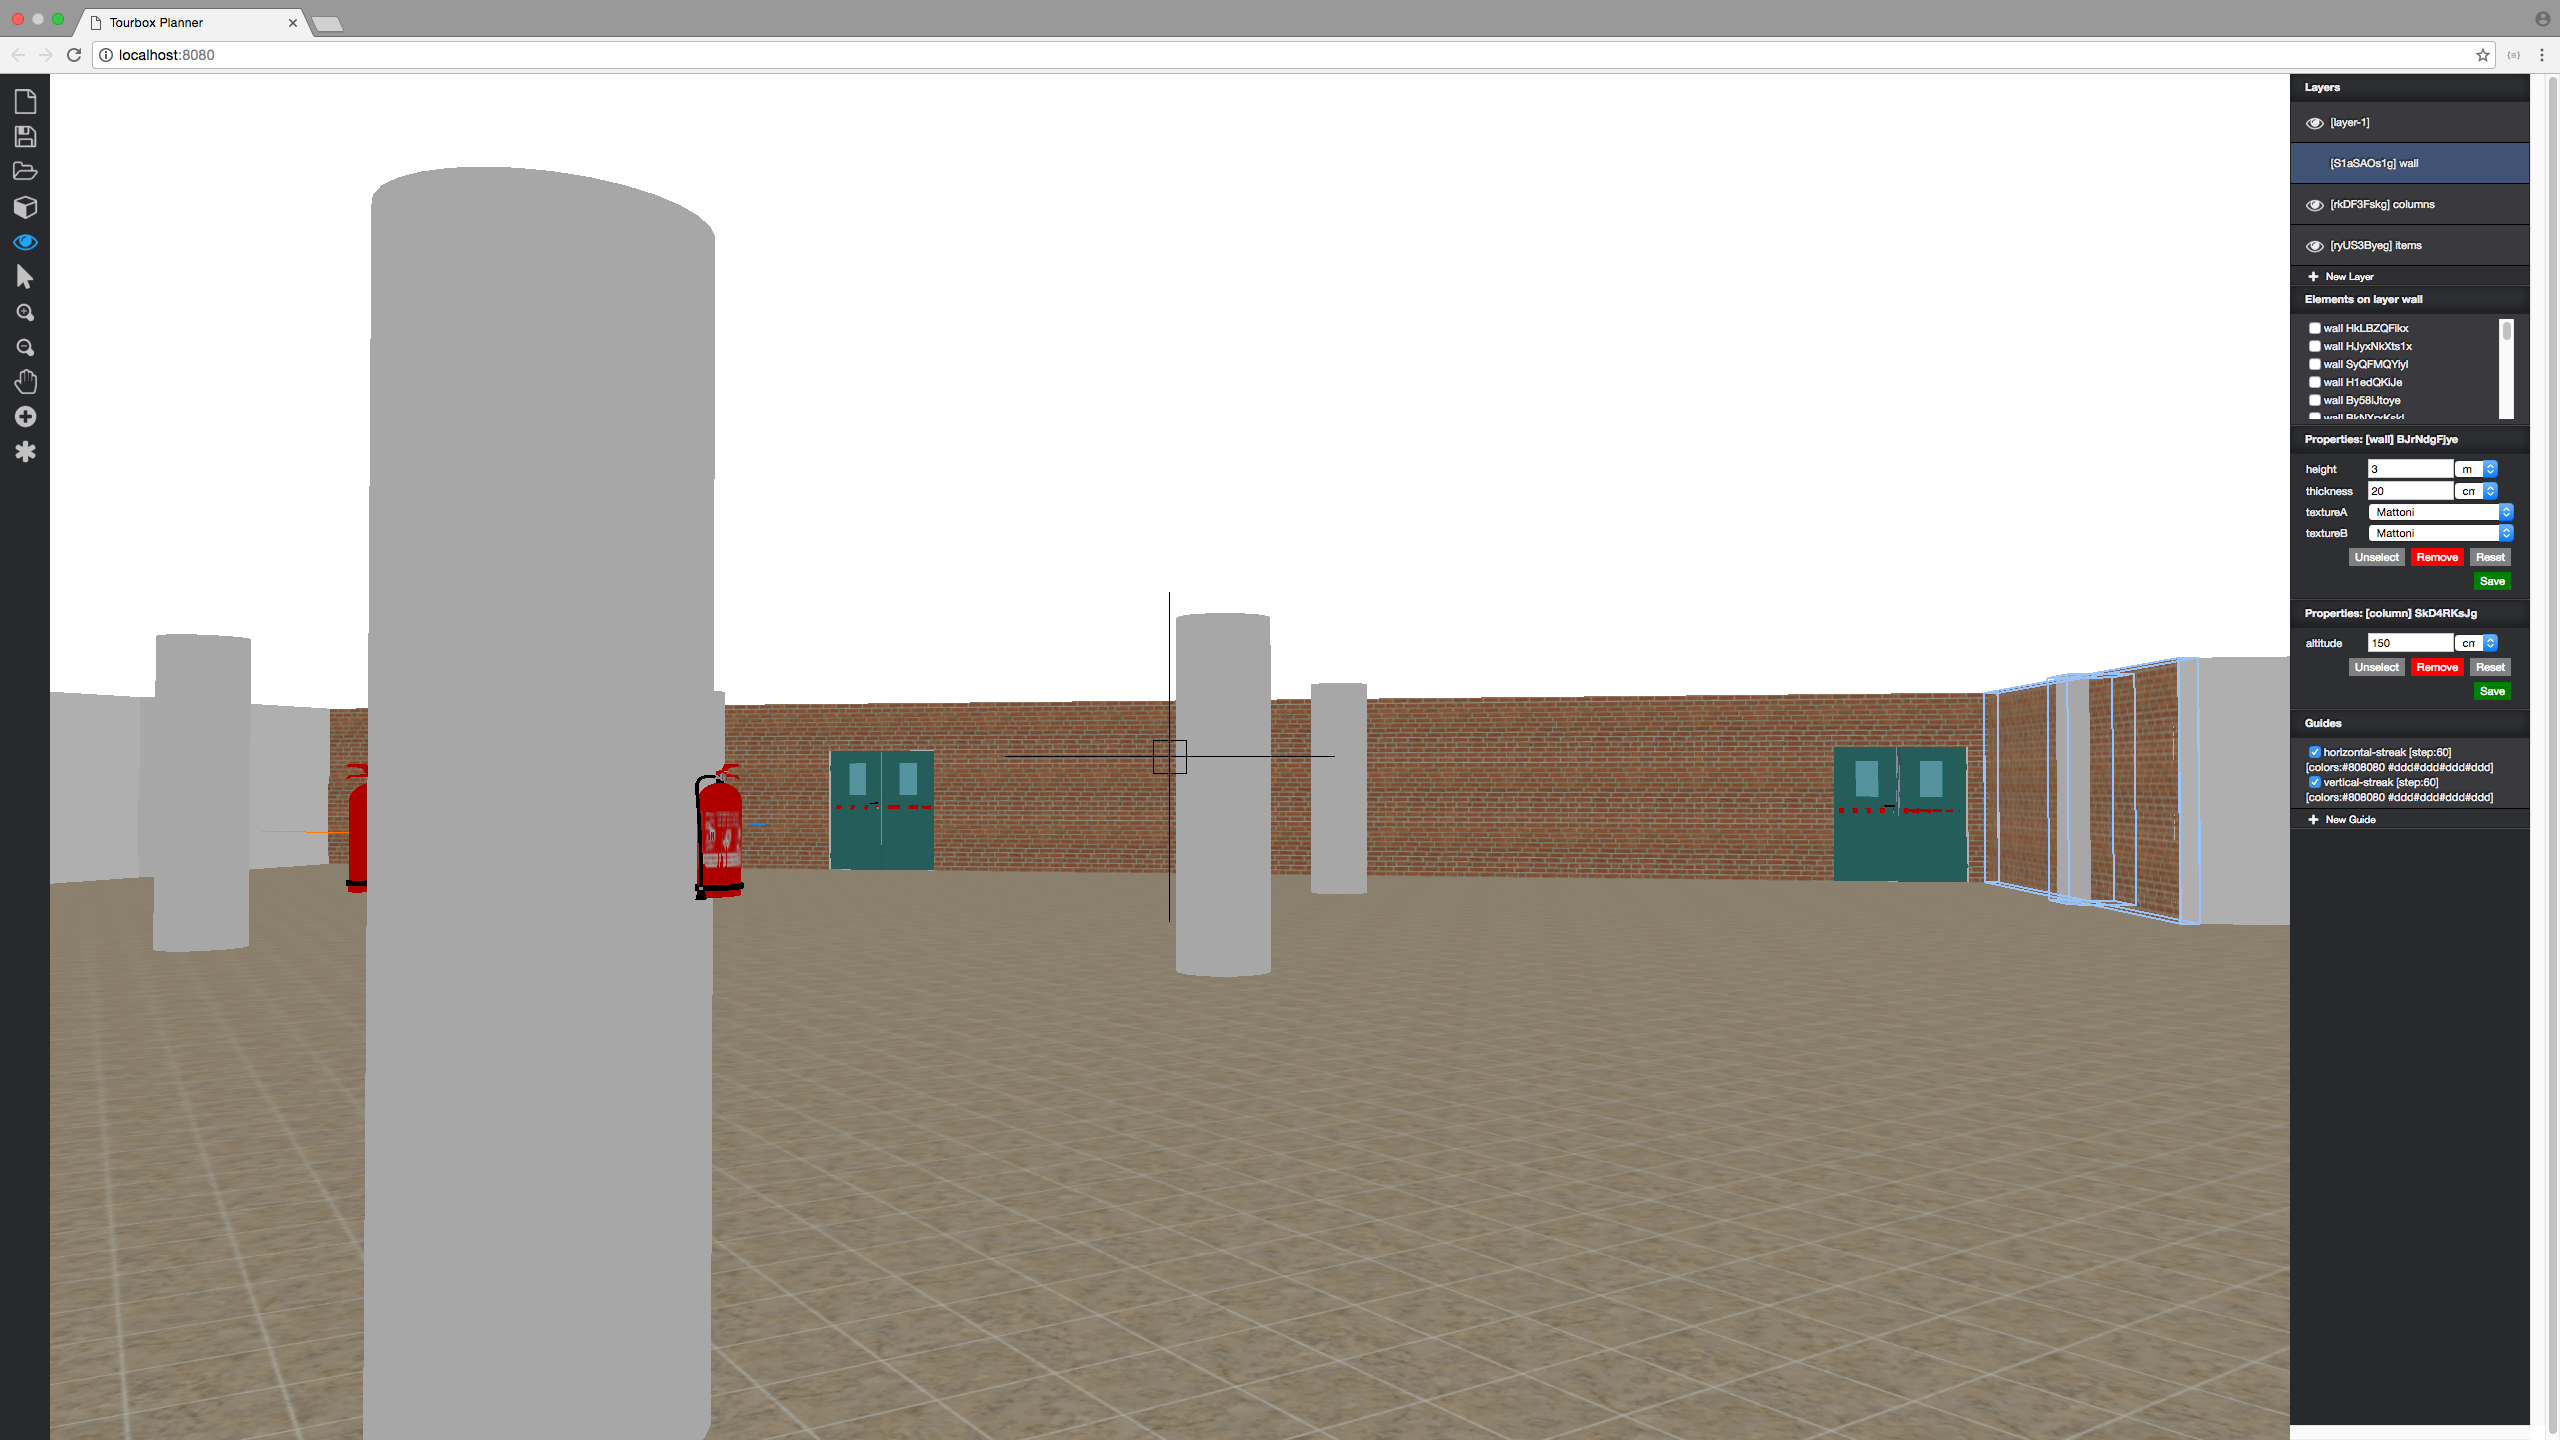
\includegraphics[width=1\linewidth]{images/ui}

   \caption{\emph{Meteor} user interface}
   \label{fig:ui}
\end{figure}

L'interfaccia utente si compone di 3 aree principali:
- toolbar
- canvas
- sidebar

Dalla toolbar � possibile richiamare le funzionalit� per:
- gestire il ciclo di vita di un progetto (nuovo, carica, salva),
- editare il progetto (aprire il catalogo di elementi architetturali da disegnare)
- cambiare la modalit� di visualizzazione (2D \& 3D)
- cambiare le modalit� di interazione (pan \& zoom)

La canvas presenta il progetto nelle differenti modalit� di visualizzazione
- modalit� 2D, vista dall'alto, in cui � possibile inserire/selezionare elementi
- modalit� 3D, vista esterna prospettica o ortografica, in cui e possibile selezionare elementi
- modalit� 3D, vista in prima person, in cui � possibile navigare il progetto

La sidebar presenta le propriet� specifiche dell'elemento correntemente selezionato.
Attraverso tale pannello � possibile visualizzare la descrizione dell'elemento,
modificare le propriet� dell'elemento, aggiungere/modificare/rimuovere metadati.

\subsection{Plugin-architecture}

\noindent The application has been designed to provide a small set of core interaction functionalities and to encapsulate the generation logic for architectural components (from the very basic to the most articulated) into specific plugins.

Un plugin � un componente software che pu� essere integrato nel sistema e che ne estende le capacit�.
In Metior, un plugin rappresenta un elemento architetturale che estende la capacit� di progettazione di un edificio.
Tecnicamente, un plugin rappresenta un prototipo (in programmazione orientata agli oggetti, una "classe") di un elemento architettonico, che pu� essere inserito ("instanziato") all'interno di un progetto.

\subsubsection{Definizione di un plugin}

Un plugin viene definito dalle seguenti propriet�:
\begin{itemize}
\item un nome univoco
\item una descrizione testuale
\item metadati
\item la tipologia del plugin, che pu� essere "linear", "area" o "volume"
\item le possibilit� di posizionamento del plugin, che pu� essere "inside" o "over"
\item le propriet� specifiche dell'oggetto descritto dal plugin
\item una funzione che riporta una rappresentazione 2D dell'elemento (per la vista 2D)
\item una funzione che riporta una rappresentazione 3D dell'elemento (per la vista 3D)
\end{itemize}

\subsubsection{Tassonomia dei plugin}

I plugin possono essere organizzati in base alla loro tipologia e possibilit� di posizionamento.

Gli elementi di tipo "linear" rappresentano elementi che si estendono in una dimensione (a meno di uno spessore), come ad esempio i condotti idraulici o i cavi elettrici.

Gli elementi di tipo "area" rappresentano elementi che si estendono in due dimensioni (a meno di uno spessore), ovvero gli elementi di separazione.
Questi si distinguono in "horizontal", come ad esempio i pavimenti o i solai, e "vertical", come ad esempio le pareti.

Gli elementi di tipo "volume" rappresentano elementi che si estendono nelle tre dimensioni.
Questi si distinguono in "fixed", ovvero che hanno dimensioni fisse, come ad esempio i componenti di arredo,
e "scalable", ovvero che hanno dimensioni scalabili (in modo proporzionale, o non), come ad esempio i pilastri.

Ciascun tipo determina una modalit� di instanziazione ed interazine differente, ovvero una modalit� di inserimento e di modifica dell'istanza nella canvas.
Nello specifico, nella modalit� 2D,
gli elementi di tipo "linear" sono inseriti disegnando drag\&drop linee,
gli elementi di tipo "area" sono inseriti disegnado drag\&drop il bounding-box dell'elemento,
gli elementi di tipo "volume" sono inseriti specificando point\&click la posizione dell'elemento,
e variando le sue dimensioni allargando drag\&drop il bounding-box dell'elemento.

Ciascuna possibilit� di posizionamento di un plugin determina la fattibilit� di inserimento dell'istanza del plugin all'interno della canvas.

Gli elementi di tipo "inside" possono essere inseriti solo all'interno di altri elementi di tipo "linear", "area" o "volume".
Ad esempio, una finestra � un elemento di tipo "volume inside vertical area",
un condotto idraulico pu� essere un elemento di tipo "linear inside horizontal area".

Gli elementi di tipo "over" possono essere inseriti solo a fianco di altri elementi di tipo "linear", "area" o "volume".
Ad esempio, un pilastro � un elmento di tipo "volume over horizontal area",
un pannello elettrico � un elemento di tipo "volume over vertical area".

Nella fase di progettazione, un elemento che non rispetta il vincolo definito dalla sua possibilit� di posizionamento � rilevato come warning visivo (bounding-box di colore rosso) dal sistema.

\subsubsection{Propriet� specifiche dei plugin}

Ciascun plugin ha un insieme di propriet� specifiche dell'elemento che rappresenta.
Ciascuna propriet� � definita da:
- un nome
- un tipo, che pu� essere "number", "text", "boolean", o "custom"
- un valore

Ciascun tipo di propriet� descrive e determina una modalit� di inserimento del valore specifica.
Ad esempio, un tipo "boolean" � definito da una "checkbox", un tipo "text" da una casella di testo.
Il sistema permette di definire nuovi tipi di dato, specificando l'interfaccia di inserimento del valore.
Ad esempio, un tipo "color" pu� essere definito da tre caselle numeriche che rappresentano le componenti di colore RGB,
oppure un tipo "lunghezza" pu� essere definito da una casella numerica che rappresenta il valore e da un menu a tendina
per specificare l'unit� di misura.

Le propriet� di un istanza di un plugin sono editabili dal pannello presente nella sidebar quando l'istanza � selezionata.


\subsection{Plugin Catalog}
It is pivotal to provide surveyors with a rich catalog of plugins, to cover all the basic
 as well as the most advanced modeling requirements. Built-in plugins as provided out-of-the-box by the system
 built-in
 basic
 advanced



\subsection{Server-side models generation}

\noindent Both 3D and 2D model generation has been designed to be asynchronous: the actual result of the invocation of the generation function is not the model itself but rather a \emph{promise} of the expected result. Such a design is important since the computation for model generation may require a while. In the meantime the user must be able to interact with the interface, which in turn must remain responsive. Relying on this architecture, generation of the models can be easily delegated to a server (as shown in Figure~\ref{fig:c-s-arch}), thus relieving the client from the burden of onerous computations. The server exposes a REST-like HTTP based JSON API to the client. The plugin span from the client to the server since the 2D and 3D generation functions (``3Dgf'' and ``2Dgf'' respectively in Figure~\ref{fig:c-s-arch}) defined by the plugin are actually executed on the server.

\begin{figure}[htbp] %  figure placement: here, top, bottom, or page
   \centering

   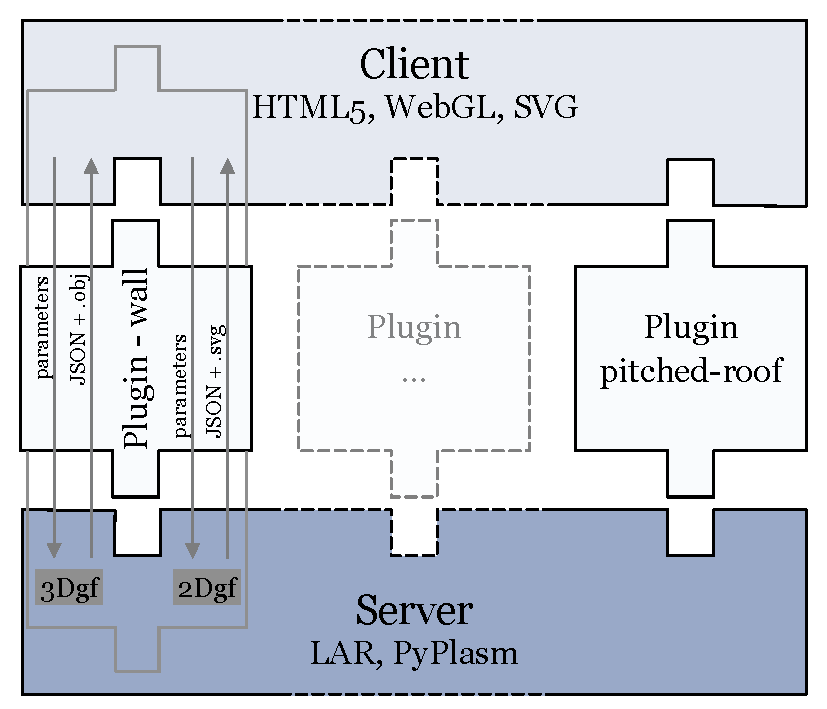
\includegraphics[width=0.6\linewidth]{images/architecture}

   \caption{Client/Server architecture for server-side models generation}
   \label{fig:c-s-arch}
\end{figure}




\noindent









